\chapter{Example Application}

In this chapter I will showcase the development of an example project that aims to demonstrate the capabilities of the selected multicore microcontroller and the Rust programming language. I will highlight features that are plain better from most perspectives, as well as the areas where this approach falls short compared to a traditional C project. The example project will have a definite function but the usage of certain peripherals and language features are more in focus thus the functionality may seem a bit purposeless as a real application.

\section{General Description}

The example application implements a very basic webserver on the M7 core of the microcontroller, and does some light signal processing on the M4 core. The general direction of this project was to design one part of the application to use the ethernet peripheral in some capacity, and the other to be capable of doing a task in real time. Also I had to make sure that safe, two-way communication between the two cores is displayed in the application.

Finally an application draft was drawn up. In it the M7 core handles the ethernet peripheral and takes on the role of a simple webserver. It hosts a simple website on a fixed IP address where coefficients of a low pass filter can be supplied. The site also displays the average value of an ADC peripheral. The other core handles the previous ADC peripheral by performs filtering with the coefficients supplied on the website and a fix formula. The filtered signal is emitted on a DAC peripheral with minimal latency latency. An average value is also calculated by the M4 core periodically from a configurable number of samples, this value will be displayed on the website.

\begin{figure}[!ht]
    \centering
    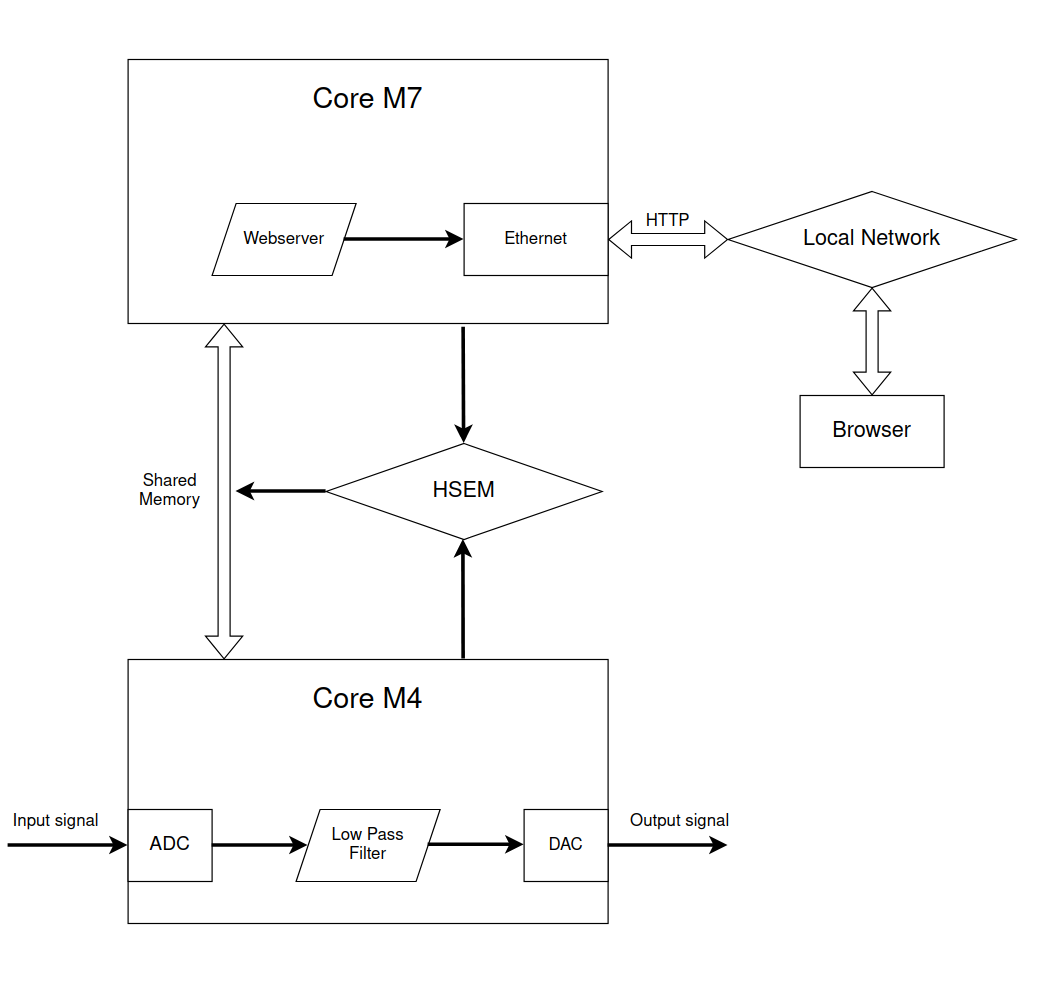
\includegraphics[width=150mm, keepaspectratio]{figures/example-app-flowchart.png}
    \caption{Block Diagram of the Example Application}
    \label{fig:app-flowchart}
\end{figure}

With this flow, the application demonstrates the usage of  a decent number of peripherals, namely an ADC, a DAC, ethernet, UART and LEDs for debugging, and of course the hardware semaphores for preventing concurrent shared memory access.

\section{Peripheral Setup}

This section demonstrates the initialization and usage of the peripherals mentioned above. Although most of these were already introduced in the previous chapter this section will focus on specific settings that facilitate this example application.

\subsection{Basic peripherals}

The basic peripherals and their usage, namely UART, LEDs, and shared memory, are already well documented in previous chapters. However some significant changes were done to the very beginning of the program where clocks, resets, and power sources are initialized. This was necessary for two reasons. For once, different clock and reset configuration was needed if we were to use the ethernet peripheral, it needed multiple types of clock signals which are supposed to be related to each other in value. The second reason was an issue where resetting the system caused it to go into an unsteady state and behave unexpectedly, eg. only one core would work. This state could only be fixed by loading a new image onto the microcontroller.

\begin{lstlisting}[language=Rust,frame=single,float=!ht,style=customrust,label={lst:clock-config},caption={Initialization of Clocks, Resets, and Power Sources}]
    let pwr = dp.PWR.constrain();
    let pwrcfg = pwr.smps().vos0(&dp.SYSCFG).freeze();

    // link SRAM3 power state to CPU1
    dp.RCC.ahb2enr.modify(|_, w| w.sram3en().set_bit());

    // Enable HSEM clk
    dp.RCC.ahb4enr.modify(|_, w| w.hsemen().set_bit());

    let rcc = dp.RCC.constrain();
    let mut ccdr = rcc
        .sys_ck(200.MHz())
        .pll1_strategy(rcc::PllConfigStrategy::Iterative)
        .pll3_p_ck(PLL3_P)
        .hclk(200.MHz())
        .pll1_r_ck(100.MHz())
        .freeze(pwrcfg, &dp.SYSCFG);

    _cp.SCB.invalidate_icache();
    _cp.SCB.enable_icache();
    _cp.DWT.enable_cycle_counter();

    assert_eq!(ccdr.clocks.hclk().raw(), 200_000_000); // HCLK 200MHz
    assert_eq!(ccdr.clocks.pclk1().raw(), 100_000_000); // PCLK 100MHz
    assert_eq!(ccdr.clocks.pclk2().raw(), 100_000_000); // PCLK 100MHz
    assert_eq!(ccdr.clocks.pclk4().raw(), 100_000_000); // PCLK 100MHz
\end{lstlisting}

In Listing~\ref{lst:clock-config} power is enabled in the usual way, then clock and power is enabled for the SRAM3 memory, which will be used by the ethernet driver, and the hardware semaphores. Then the clocks are configured according to ethernet examples from the \mycode{stm32h7xx-hal} crate. \cite{HalExamples} After that the instruction cache is flushed and enabled so every restart starts the MCU with a clean state in this regard. The last section asserts that all the clock signals are correctly configured for ethernet usage. Debugging issues around clocks would be a frustrating task when the code is already developed, so it is imperative that these asserts stop the execution if the clocks are incorrectly configured.

Some of the variable names are prepended with an underscore which signals to the Rust compiler that the variable is intentionally left unused. This may seem strange especially when a variable like this is used, but we have to remember that the code for the two diverge at some point and become separated at compile time. So if a variable is not used on one core, it will generate a warning even if the other core uses it. This solution is more acceptable then turning off unused variable warnings altogether.

\subsection{Ethernet}

In this section I will demonstrate the usage of the ethernet peripheral and its driver coupled with a TCP stack.

\subsubsection{Driver}

The ethernet driver is part of the \mycode{stm32h7xx-hal} crate. this driver provides an interface for the STM32H7 microcontroller to communicate over Ethernet using the MAC and PHY components. It leverages DMA for efficient data transfer and integrates with the \mycode{smoltcp} crate, which will serve as the TCP stack, to enable networking capabilities. The driver can be used for tasks such as sending and receiving Ethernet frames, configuring MAC and PHY parameters, and interfacing with higher-level networking protocols.

The driver provides an \mycode{EthernetMAC} struct which represents the MAC (Media Access Control) layer. It initializes and configures the MAC for communication by setting up its registers. These hold various information handled by this layer such as MAC address and flow control settings. It also provides methods \mycode{smi_read()} and \mycode{smi_write()} for the SMI (Serial Management Interface) which facilitates the communication between the MAC and the external PHY registers. these methods are provided by implementing the \mycode{StationManagement} trait for the \mycode{EthernetMAC} struct.

DMA is extensively used by the ethernet driver so the CPU is not throttled by the constant flow of information that is typical to this interface. The \mycode{EthernetDMA} struct represents the Ethernet DMA engine which is responsible for managing the flow of data between memory and the MAC.
DMA descriptors, \mycode{TDes} and \mycode{RDes}, are used to control the transfer of data between the MAC and memory. The descriptors are organized in rings for efficient handling of multiple data frames. The \mycode{TDesRing} and \mycode{RDesRing} structs manage the transmit and receive descriptor rings, respectively. The \mycode{init()}, \mycode{available()}, \mycode{release()}, and \mycode{buf_as_slice_mut()} methods provide functionality for initializing, checking availability, releasing, and accessing DMA descriptors and associated buffers.

\subsubsection{Smoltcp}

The \mycode{smoltcp} crate stands as a versatile networking stack in the Rust programming language, designed to offer modularity and composability for the development of networking applications. At its core, \mycode{smoltcp} supports a range of essential networking protocols such as IPv4, IPv6, TCP, UDP, ICMP, and more. In this project, \mycode{smoltcp} is primarily used as a TCP stack in the networking schema. \cite{Smoltcp}

One of the key architectural principles of \mycode{smoltcp} lies in its abstraction of networking devices through the \mycode{phy::Device} trait. This trait serves as the interface for network devices, allowing seamless integration with different hardware or software networking implementations. This level of abstraction enhances the adaptability of \mycode{smoltcp} to various platforms and facilitates ease of use.

A notable aspect of the crate is its adherence to the Berkeley Sockets API, providing a familiar programming interface for developers well-versed in network programming. This socket API simplifies the process of building networking applications, contributing to a smoother development experience.

Still, one of the main reasons \mycode{smoltcp} is used in embedded projects like this is that is can operate using a \mycode{no_std} environment, and still being able to provide fairly high level API-s.

\subsubsection{Connection to TCP stack}

The connection to the \mycode{smoltcp} crate, which servers as the TCP stack in this project, is achieved by implementing the \mycode{phy::Device} trait. The driver does this and so \mycode{smoltcp} is able to communicate with the underlying network device. There are two other interfaces that need implementation before our program can fully utilize the TCP stack.

First of all a static storage is needed to store various data. In this project Listing~\ref{lst:static-net-storage} fills this function. Most notably it can hold IP addresses, sockets, and routes, while also providing the TX and RX buffers for the TCP stack.

\begin{lstlisting}[language=Rust,frame=single,float=!ht,style=customrust,label={lst:static-net-storage},caption={Definition of Net Static Storage Type}]
    #[cfg(core = "0")]
    pub struct EthernetStorage<'a> {
        ip_addrs: [IpCidr; 1],
        socket_storage: [SocketStorage<'a>; 8],
        neighbor_cache_storage: [Option<(IpAddress, Neighbor)>; 8],
        routes_storage: [Option<(IpCidr, Route)>; 1],

        // network buffers
        tcp_rx_buffer_storage: [u8; MAX_PACKET_SIZE],
        tcp_tx_buffer_storage: [u8; MAX_PACKET_SIZE],
    }
\end{lstlisting}

The static storage is only the first part of the puzzle. We also need to implement the \mycode{Interface} trait from the \mycode{smoltcp} crate which consists of two functions. The \mycode{new()} function will create an instance of \mycode{Net}, which is the name for our implementation of \mycode{Interface}, by populating the previously defined static storage. The \mycode{pull()} method will poll the ethernet interface and load the RX buffers when it is triggered. It can be triggered by explicitly calling the method, or what is used in this case, a dedicated ethernet interrupt.

\begin{lstlisting}[language=Rust,frame=single,float=!ht,style=customrust,label={lst:eth-interrup-handler},caption={Ethernet Interrupt Handler}]
    #[cfg(core = "0")]
    #[interrupt]
    fn ETH() {
        unsafe { ethernet::interrupt_handler() };

        if let Some(ethernet) = unsafe { ETHERNET.as_mut() } {
            let time = ATOMIC_TIME.load(Ordering::Relaxed);
            ethernet.poll(time as i64);
        }
    }
\end{lstlisting}

\subsubsection{Usage}

Before we can start using the ethernet peripheral we first need to instantiate the types we defined before.

\begin{lstlisting}[language=Rust,frame=single,float=!ht,style=customrust,label={lst:eth-globals},caption={Global Static Variables Related to Ethernet}]
    const MAC_LOCAL: [u8; 6] = [0x02, 0x00, 0x11, 0x22, 0x33, 0x44];
    const IP_LOCAL: [u8; 4] = [192, 168, 0, 139];
    const MAX_PACKET_SIZE: usize = 576;
    const LOCAL_PORT: u16 = 6970;

    static ATOMIC_TIME: AtomicU32 = AtomicU32::new(0);
    static mut ETHERNET: Option<Net> = None;
    static mut ETHERNET_STORAGE: EthernetStorage = EthernetStorage::new();
    #[link_section = ".sram3.eth"]
    static mut ETHERNET_DESCRIPTOR_RING: ethernet::DesRing<4, 4> = ethernet::DesRing::new();
\end{lstlisting}

The first part of Listing~\ref{lst:eth-globals} contains global constants that are related to. Notice that an IP address needs to be set here because in this configuration the network stack uses a static IP address. MAC address and port can also be set here. From these settings it can be inferred that the webserver will host the website on the local address, \url{http://192.168.0.1:6970}.

The second part is more interesting. Here, the global ethernet object and the ethernet storage it uses are created. An ethernet descriptor ring is also needed to facilitate DMA transfers. With the \mycode{#[link_section = ".sram3.eth]}, it can be placed in a specific section of SRAM3 which is defined by the HAL crate.

Next, the ethernet peripheral can finally be initialized with all types and variables being defined. After the correct pins assume their appropriate modes, DNA and MAC objects are created from the static variables.

\begin{lstlisting}[language=Rust,frame=single,float=!ht,style=customrust,label={lst:eth-init},caption={Initialization of the Ethernet Peripheral}]
    let mac_addr = EthernetAddress::from_bytes(&MAC_LOCAL);
    let (eth_dma, eth_mac) = unsafe {
        ethernet::new_unchecked(
            dp.ETHERNET_MAC,
            dp.ETHERNET_MTL,
            dp.ETHERNET_DMA,
            &mut ETHERNET_DESCRIPTOR_RING,
            mac_addr.clone(),
            ccdr.peripheral.ETH1MAC,
            &ccdr.clocks,
        )
    };

    let mut lan8742a = ethernet::phy::LAN8742A::new(eth_mac.set_phy_addr(0));
    lan8742a.phy_reset();
    lan8742a.phy_init();
    while !lan8742a.poll_link() {}

    unsafe {
        ethernet::enable_interrupt();
        _cp.NVIC.set_priority(pac::Interrupt::ETH, 196); // mid prio
        cortex_m::peripheral::NVIC::unmask(pac::Interrupt::ETH);
    }

    unsafe { ETHERNET = Some(Net::new(&mut ETHERNET_STORAGE, eth_dma, mac_addr)); }
\end{lstlisting}

After that, a handler for the PHY is created and used for resetting and initializing the layer. The program then busy waits for the link to become active. At this point the interface is ready to be used but the global ethernet object needs to be populated with relevant references, and the ethernet interrupt needs to be enabled. This is done in the last and second to last parts of Listing~\ref{lst:eth-init}.

As a final step, some references are created in the TCP stack.

\begin{lstlisting}[language=Rust,frame=single,float=!ht,style=customrust,label={lst:tcp-init},caption={Creating References for TCP Objects}]
    let store = unsafe { &mut ETHERNET_STORAGE };
    let tcp_rx_buffer = TcpSocketBuffer::new(&mut store.tcp_rx_buffer_storage[..]);
    let tcp_tx_buffer = TcpSocketBuffer::new(&mut store.tcp_tx_buffer_storage[..]);
    let tcp_socket_handle = unsafe { ETHERNET.as_mut().unwrap().interface.add_socket(TcpSocket::new(tcp_rx_buffer, tcp_tx_buffer)) };
\end{lstlisting}

\subsection{ADC}

Initializing the ADC is not as cumbersome as setting up ethernet was, it does not require any additional setup. We only need to create a handle with which the peripheral can be configured.

\begin{lstlisting}[language=Rust,frame=single,float=!ht,style=customrust,label={lst:adc-init},caption={Initialization of the ADC}]
    let mut adc1 = adc::Adc::adc1(
        dp.ADC1,
        16.MHz(),
        &mut delay,
        ccdr.peripheral.ADC12,
        &ccdr.clocks,
    ).enable();
    adc1.set_resolution(adc::Resolution::SixteenBit);
    let mut channel = gpioc.pc0.into_analog();
\end{lstlisting}

We are using the ADC1 peripheral but it is not coupled with ADC2 in this instance. Sampling time is set at 16 MHz and the resolution is sixteen bit. The channel is implicitly selected by defining which physical pin is used as analog input.

\subsection{DAC}

Configuring the DAC is an even more simple task. We only need to acquire a handler for the DAC instance, which covers both DAC modules, and calibrate the buffer. This way the default settings are used, which means that the output can be given in a 12 bit format, making the minimal value \mycode{0} and the maximal \mycode{4095}.

\begin{lstlisting}[language=Rust,frame=single,float=!ht,style=customrust,label={lst:dac-init},caption={Initialization of the DAC}]
    let dac = dp.DAC.dac(gpioa.pa4, ccdr.peripheral.DAC12);
    let mut dac = dac.calibrate_buffer(&mut delay).enable();
    dac.set_value(2048);
\end{lstlisting}

The last line of Listing~\ref{lst:dac-init} the output value is set to the 50\% of VDDA which is configured to be 3.3 V by default.

\section{Main Loop}

In this section I will showcase what the two cores are doing after their initialization is complete and enter their respective infinite loops.

\subsection{Webserver}

On the M7 core a very minimalist webserver is implemented. The server will basically wait for a GET or POST HTTP request and send back an answer containing a simple HTML website.

\begin{lstlisting}[language=Rust,frame=single,float=!ht,style=customrust,label={lst:html-strings},caption={HTML Page Defined in a String}]
    const WEBPAGE_UPPER: &str =
    "HTTP/1.1 200 OK
    Content-Type: text/html

    <!DOCTYPE html>
    <html>
    <head>
        <title>STM32H745 Dual Core Demo App</title>
    </head>
    <body>
        <h1>STM32H745 Dual Core Demo App</h1>";

    const WEBPAGE_LOWER: &str =
    r#"
    <p>The filtering will use the formula: y[0] = alpha*u[0]+(1-alpha)*y[-1] + beta*u[-1]
    <form action="/" method="POST">
      <input type="text" id="alpha" name="alpha" placeholder="alpha">
      <input type="text" id="beta" name="beta" placeholder="beta">
      <input type="submit" value="Set">
    </form>
    </body>
    </html>"#;
\end{lstlisting}

\begin{figure}[!ht]
    \centering
    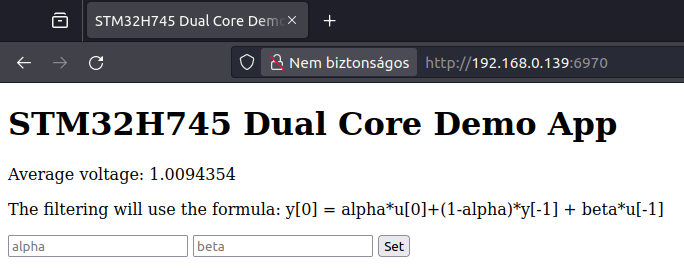
\includegraphics[width=150mm, keepaspectratio]{figures/webpage.png}
    \caption{Screenshot of the HTML Page}
    \label{fig:html-page}
\end{figure}

The HTML page is broken into an upper and lower part. The middle can contain additional elements, for example the average value will be displayed this way. Besides that, it has a title and a form in which an alpha and a beta value can be provided. How these coefficients influence the filtering done on the other core is also displayed on the page.

As with any server using sockets, the loop of this one starts with entering a \mycode{listen()} function. Once a connection is established, the server can call a \mycode{recv()} function. The data can be received in a closure, where it can be collected into a byte array.

\begin{lstlisting}[language=Rust,frame=single,float=!ht,style=customrust,label={lst:server-recv},caption={Receiving the Contents of the TCP Buffer}]
    if !tcp_socket.is_open() {
        tcp_socket.listen(LOCAL_PORT).unwrap();
    }

    if tcp_socket.may_recv() {
        let mut headers = [httparse::EMPTY_HEADER; 16];
        let mut req = httparse::Request::new(&mut headers);
        let mut data_len = 0;
        let display_voltage;
        let data = tcp_socket.recv(|buffer| {
            let mut data = [0u8; 576];
            data_len = buffer.len();
            for i in 0..buffer.len() {
                data[i] = buffer[i];
            }
            (buffer.len(), data)
        }).unwrap();

    // ...
\end{lstlisting}

After this the data needs to be parsed. We know that it contains an HTML request. For parsing the header part of the request, an external crate, \mycode{httparse} can be used. This crate is compatible with projects that do not use the standard library, as it does not allocate memory other than the buffer it receives the data in. \cite{Httparse} After parsing the HTTP header, all of its records are available, but here we only need the type of the request. For GET requests, the server will simply send back the HTML page to the client and close the connection. POST requests are used to update the values of the alpha and beta coefficients. The HTML page is included in the reply to the POST request too. The route of the request is not checked, so this server currently can only supply this single page, but does not require routing. All the other type of HTTP requests just cause the server to close the connection.

\begin{lstlisting}[language=Rust,frame=single,float=!ht,style=customrust,label={lst:get-post},caption={Handling of GET and POST requests}]
    let hsem_taken_by_this_core = 0x80000000u32 & ((get_core_id() as u32) << 8);
    let _res = req.parse(&data).unwrap();
    match req.method.unwrap() {
        "GET" => {
            log_serial!(tx, "In GET arm\r\n");
            hsem.r[0].read().lock().bit();
            delay.delay_ms(100u16);
            hsem.r[0].write(|w| unsafe { w
                .procid().bits(0)
                .masterid().bits(3)
                .lock().bit(false) }
            );
        }
        "POST" => {
            log_serial!(tx, "In POST arm\r\n");
            (alpha, beta) = extract_coefs(&data);
            log_serial!(tx, "Got {} and {}\r\n", alpha, beta);
            while hsem.fast_lock(0).unwrap() != hsem_taken_by_this_core {}
            unsafe {
                display_voltage = SHARED_DATA.voltage;
                SHARED_DATA.alpha = alpha;
                SHARED_DATA.beta = beta;
            }
            let _ = hsem.release(0);
        }
        _ => {
            log_serial!(tx, "In ERROR arm\r\n");
            tcp_socket.close();
        }
    }
\end{lstlisting}

The variables set in a POST request are stored in the body of the request in the format \mycode{variable1=value1&variable2=value2} and so on. These are extracted by a function that parses the body of the HTTP request. Then the hardware semaphore is taken and alpha and beta can be placed in a shared memory region, while the average voltage supplied by the other core can be extracted and prepped for display in the next step.

If the server is able to send to the client it will write the HTML page into the TCP TX buffer and send it before closing the connection. The average voltage is placed between the upper and lower parts of the page with the help of the \mycode{format_args!()} macro.

\begin{lstlisting}[language=Rust,frame=single,float=!ht,style=customrust,label={lst:may-send},caption={Sending a Response to the Client}]
    if tcp_socket.may_send() {
        let webpage = write_to::show(&mut webpage,
            format_args!("{}Average voltage: {}{}", WEBPAGE_UPPER, display_voltage, WEBPAGE_LOWER))
            .unwrap()
            .as_bytes();
        tcp_socket.send_slice(webpage).unwrap();
        tcp_socket.close();
    }
\end{lstlisting}

With the connection closed, the job of this core is done and the loop can start again from the beginning with the listening phase.

\subsection{Signal Filtering}
